\chapter{Accesso a Passi, B-Tree e Impatto della Paginazione Virtuale}
\label{cha:lecture-two}

\begin{center}
  \textbf{Lezione 2}\\
  \emph{Accesso a passi, ricerca binaria contro B-Tree e paginazione virtuale}\\[0.5em]
  Data: 16 settembre 2026
\end{center}

Questo capitolo studia come il pattern di accesso di un algoritmo interagisca con la granularità di trasferimento di un sistema di memoria. Lo stesso lavoro aritmetico può avere costi molto differenti a seconda che gli accessi preservino la località spaziale, corrispondano alla dimensione del blocco, o superino la capacità della memoria veloce.

\section{Accesso Non Sequenziale: L'Algoritmo \texorpdfstring{$A_{s,b}$}{A-s-b}}
\label{sec:strided-access}

Sia $S$ un array contenente $n$ elementi. Il sistema di archiviazione trasferisce i dati in blocchi fisici di dimensione $B$ (un blocco del disco o una linea di cache). Definiamo inoltre una dimensione del blocco logico $b$, dove $b \leq B$ e $b$ divide $B$. I corrispondenti numeri di blocchi logici e fisici sono
\[
  N' = \frac{n}{b},
  \qquad
  N_{\mathrm{phys}} = \frac{n}{B}.
\]

L'algoritmo $A_{s,b}$ calcola la somma degli elementi visitando i blocchi logici con un pattern a passi (stride). Il blocco logico visitato al passo $j$ è
\[
  \operatorname{block}(j) = (j s) \bmod N',
  \qquad j = 0,1,\ldots,N'-1.
\]

\subsection{Condizione di Coprimalità}
\label{subsec:coprimality}

La sequenza visita ogni blocco logico esattamente una volta se e solo se
\[
  \gcd\!\left(s,\frac{n}{b}\right)=1.
\]
In tal caso, la moltiplicazione per $s$ è una permutazione dei residui modulo $N'$. Se il massimo comun divisore è $d>1$, la sequenza si ripete dopo $N'/d = n/(bd)$ blocchi logici distinti e di conseguenza copre solo una frazione dell'array.

\begin{figure}[htbp]
  \centering
  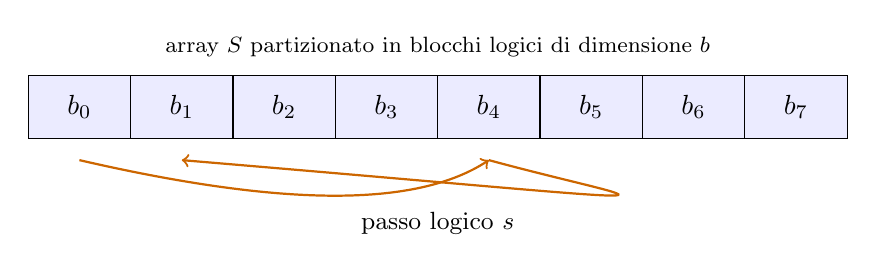
\begin{tikzpicture}[x=13mm,y=8mm]
    \foreach \i in {0,...,7} {
      \draw[fill=blue!8] (\i,0) rectangle ++(1,1);
      \node at (\i+0.5,0.5) {$b_{\i}$};
    }
    \draw[->,thick,orange!80!black] (0.5,-0.35) .. controls (2.5,-1.1) and (3.8,-1.1) .. (4.5,-0.35);
    \draw[->,thick,orange!80!black] (4.5,-0.35) .. controls (6.2,-1.1) and (7.0,-1.1) .. (1.5,-0.35);
    \node[font=\small] at (4,-1.35) {passo logico $s$};
    \node[font=\footnotesize,align=center] at (4,1.45)
      {array $S$ partizionato in blocchi logici di dimensione $b$};
  \end{tikzpicture}
  \caption{Un passo modulare visita i blocchi logici in un ordine non sequenziale.}
  \label{fig:logical-stride}
\end{figure}

La \autoref{fig:logical-stride} illustra l'ordine logico degli accessi. Il costo fisico dipende da come questo ordine si mappa su blocchi di dimensione $B$, piuttosto che unicamente dal numero di operazioni aritmetiche.

\subsection{Costo di I/O}
\label{subsec:stride-io}

Una prima utile approssimazione confronta la distanza fisica tra accessi logici successivi, $s b$, con la dimensione del blocco fisico $B$.

\begin{table}[htbp]
  \centering
  \caption{Comportamento approssimato di I/O del pattern di accesso a passi.}
  \label{tab:stride-io}
  \begin{tabularx}{\textwidth}{@{}p{0.25\textwidth}YY@{}}
    \toprule
    Condizione & Località e comportamento & Costo di I/O \\
    \midrule
    $s b < B$ & Diversi accessi logici possono condividere un singolo blocco fisico; una parziale località spaziale è preservata. & $\Theta(n/B)$ \\
    $s b \geq B$ & Gli accessi successivi tipicamente ricadono su blocchi fisici differenti. Se $M<n$, il working set non può rimanere interamente nella memoria veloce. &
      $\Theta(n/b)$ \\
    $b=1$ e $s\geq B$ & Ogni accesso logico è un singolo elemento e il passo distrugge il beneficio dei trasferimenti a blocchi. & $\Theta(n)$ \\
    \bottomrule
  \end{tabularx}
\end{table}

I limiti nella \autoref{tab:stride-io} descrivono il tipico regime del caso pessimo o dei capacity miss. Le costanti esatte dipendono dall'allineamento, dalla politica di rimpiazzo e dall'interazione tra la sequenza modulare e i blocchi fisici. Nell'ultimo caso, il costo è peggiore di un fattore pari a circa $B$ rispetto ad una scansione lineare, che può sfruttare ogni elemento trasferito.

\section{Limiti Algoritmici e Accelerazione Hardware}
\label{sec:scaling-laws}

Fissiamo un tempo di esecuzione massimo ammissibile $T_0$ e assumiamo che l'hardware o il parallelismo accelerino il calcolo di un fattore $K$. La macchina accelerata può pertanto permettersi un tempo di esecuzione originale pari a
\[
  \frac{T(n)}{K}=T_0
  \qquad\Longleftrightarrow\qquad
  T(n)=K T_0.
\]
L'effetto sulla dimensione massima dell'input risolvibile dipende dal tasso di crescita di $T$.

\begin{table}[htbp]
  \centering
  \small
  \caption{Effetto di un'accelerazione hardware di un fattore $K$ sulla dimensione dell'input risolvibile.}
  \label{tab:scaling-laws}
  \begin{tabularx}{\textwidth}{@{}p{0.15\textwidth}p{0.19\textwidth}YY>{\raggedright\arraybackslash}p{0.18\textwidth}@{}}
    \toprule
    Algoritmo & Complessità & Hardware di base & Hardware accelerato & Guadagno effettivo \\
    \midrule
    $A_1$ & $c n$ & $n_1=T_0/c$ & $n'_1=K n_1$ & Moltiplicativo, $K$ \\
    $A_2$ & $c n^2$ & $n_2=\sqrt{T_0/c}$ & $n'_2=\sqrt{K}\,n_2$ & Sublineare, $\sqrt K$ \\
    $A_3$ & $c2^n$ & $n_3=\log_2(T_0/c)$ & $n'_3=n_3+\log_2 K$ & Additivo, $+\log_2 K$ \\
    \bottomrule
  \end{tabularx}
\end{table}

\begin{figure}[htbp]
  \centering
  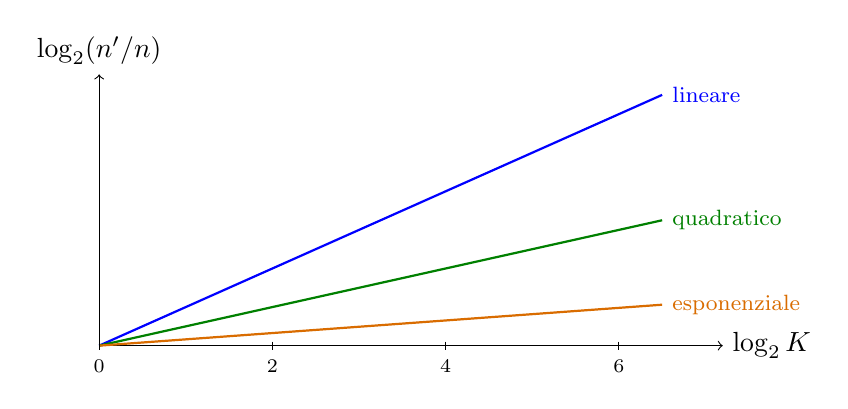
\begin{tikzpicture}[x=1.1cm,y=0.65cm]
    \draw[->] (0,0) -- (7.2,0) node[right] {$\log_2 K$};
    \draw[->] (0,0) -- (0,5.3) node[above] {$\log_2(n'/n)$};
    \draw[thick,blue] (0,0) -- (6.5,4.9) node[right,font=\footnotesize] {lineare};
    \draw[thick,green!50!black] (0,0) -- (6.5,2.45) node[right,font=\footnotesize] {quadratico};
    \draw[thick,orange!85!black] (0,0) -- (6.5,0.8) node[right,font=\footnotesize] {esponenziale};
    \foreach \x/\label in {0/0,2/2,4/4,6/6} {
      \draw (\x,0.08) -- (\x,-0.08) node[below,font=\scriptsize] {\label};
    }
  \end{tikzpicture}
  \caption{Beneficio relativo dell'accelerazione hardware per tassi di crescita rappresentativi.}
  \label{fig:scaling-laws}
\end{figure}

La \autoref{fig:scaling-laws} mostra perché i miglioramenti hardware non rimuovono un algoritmo asintoticamente inefficiente. Per un algoritmo esponenziale, persino uno speedup di $1000$ volte aumenta la dimensione dell'input risolvibile di soli $\log_2(1000)\approx 10$ elementi.

\section{Ricerca in Insiemi Ordinati: Ricerca Binaria contro B-Tree}
\label{sec:binary-search-btrees}

\subsection{Ricerca Binaria in Memoria Secondaria}
\label{subsec:external-binary-search}

Per una sequenza ordinata di $n$ chiavi memorizzate in blocchi di dimensione $B$, la ricerca binaria esegue $\Theta(\log_2 n)$ confronti sulla CPU. Il suo costo di I/O è maggiore di quanto il numero di confronti suggerisca: durante le prime iterazioni, le posizioni esaminate sono separate da $n/2$, $n/4$ e così via. Finché l'intervallo di ricerca non si restringe ad al più $B$ elementi, ogni sondaggio può indirizzare un blocco fisico differente. Pertanto,
\[
  \operatorname{I/O}_{\mathrm{ricerca\ binaria}}
  \approx \log_2 n-\log_2 B
  = \log_2\!\left(\frac{n}{B}\right).
\]
L'approssimazione ignora l'allineamento e la possibilità che un blocco rimanga nella cache, ma cattura il comportamento dominante in memoria esterna.

\subsection{B-Tree e \texorpdfstring{B$^+$-Tree}{B+-Tree}}
\label{subsec:btree}

Un B-Tree sceglie la dimensione del nodo in modo che corrisponda ad un blocco fisico. Ogni nodo memorizza $\Theta(B)$ chiavi e puntatori ai figli, pertanto il suo fan-out è $\Theta(B)$. Un B$^+$-Tree usa lo stesso principio e normalmente memorizza i record o i puntatori ai record nelle sue foglie, rendendolo particolarmente adatto per le query ad intervallo.

\begin{figure}[htbp]
  \centering
  \begin{tikzpicture}[
    nodebox/.style={draw,rounded corners=2pt,minimum height=8mm,align=center,font=\small},
    edge/.style={-Latex,thick},
    level distance=13mm,
    sibling distance=27mm
  ]
    \node[nodebox,fill=blue!12] (root) {[K$_1$ \textbar K$_2$ \textbar K$_3$]\\blocco radice};
    \node[nodebox,fill=green!10,below left=of root] (left) {blocco figlio};
    \node[nodebox,fill=green!10,below=of root] (middle) {blocco figlio};
    \node[nodebox,fill=green!10,below right=of root] (right) {blocco figlio};
    \draw[edge] (root) -- (left);
    \draw[edge] (root) -- (middle);
    \draw[edge] (root) -- (right);
    \node[font=\footnotesize,below=7mm of middle] {ogni nodo occupa approssimativamente un blocco fisico $B$};
  \end{tikzpicture}
  \caption{Un B-Tree orientato ai blocchi con alto fan-out.}
  \label{fig:btree}
\end{figure}

La \autoref{fig:btree} mostra la decisione fondamentale di layout: un I/O carica un intero nodo e fornisce molte chiavi di instradamento e puntatori. L'altezza, e di conseguenza il numero di letture di blocchi per una point query, è approssimativamente
\[
  h = \log_B\!\left(\frac{n}{B}\right)
    = \frac{\log_2(n/B)}{\log_2 B}.
\]
Più precisamente, i dettagli implementativi introducono arrotondamenti per eccesso e fattori di occupazione. Lo spazio dei nodi interni è piccolo in confronto a quello delle foglie poiché
\[
  \text{nodi interni}
  \leq \frac{n}{B^2}+\frac{n}{B^3}+\cdots
  = \frac{n}{B(B-1)}
  \ll \frac{n}{B}.
\]

\subsection{Confronto Quantitativo}
\label{subsec:btree-comparison}

Ignorando gli arrotondamenti per eccesso, lo speedup di I/O di un B-Tree rispetto alla ricerca binaria è
\[
  \frac{\operatorname{I/O}_{\mathrm{ricerca\ binaria}}}
       {\operatorname{I/O}_{\mathrm{B\text{-}Tree}}}
  = \frac{\log_2(n/B)}{\log_2(n/B)/\log_2 B}
  = \log_2 B.
\]

\begin{table}[htbp]
  \centering
  \caption{Confronto illustrativo per un grande dataset ordinato.}
  \label{tab:btree-example}
  \begin{tabularx}{\textwidth}{@{}lX@{}}
    \toprule
    Parametro & Valore \\
    \midrule
    Dimensione del dataset & $n=2^{40}$ elementi, approssimativamente $10^{12}$ record \\
    Dimensione del blocco & $B=2^{14}=16\,384$ record \\
    I/O della ricerca binaria & $40-14=26$ accessi ai blocchi \\
    I/O del B-Tree & $(40-14)/14\approx1.85$, quindi circa $2$ accessi ai blocchi \\
    \bottomrule
  \end{tabularx}
\end{table}

Per una latenza di archiviazione su scala dei millisecondi, la differenza tra approssimativamente $26$ e $2$ accessi ai blocchi cambia una point query da centinaia di millisecondi a soli pochi millisecondi, subordinatamente alla cache e ai dettagli hardware.

\section{Algoritmi I/O-Aware e Paginazione Virtuale}
\label{sec:paging}

Ci sono due modi complementari per gestire i trasferimenti tra memoria veloce e lenta:

\begin{description}
  \item[Progettazione I/O-aware (esplicita).] L'algoritmo modella $B$ e la capacità della memoria veloce $M$ in modo diretto, e gestisce buffer, layout dei dati e trasferimenti in modo programmatico.
  \item[Memoria virtuale e paginazione (implicita).] Il sistema operativo e l'hardware muovono le pagine in modo trasparente utilizzando tabelle delle pagine e politiche di rimpiazzo come le approssimazioni LRU.
\end{description}

\subsection{Paginazione con un Working Set Sovradimensionato}
\label{subsec:paging-model}

Assumiamo che la memoria fisica abbia capacità $M$ e sia divisa in $M/B$ frame. Se l'applicazione richiede
\[
  n=(1+\varepsilon)M=M+\varepsilon M,
  \qquad \varepsilon>0,
\]
allora almeno $\varepsilon M$ unità del working set devono risiedere nella memoria secondaria. Sia $\alpha$ la frazione di istruzioni che eseguono operazioni di memoria. Un tipico profilo di istruzione è:

\begin{itemize}
  \item frazione $1-\alpha$: operazioni aritmetiche o logiche, con costo di circa un ciclo di CPU;
  \item frazione $\alpha$: operazioni \texttt{LOAD} o \texttt{STORE};
  \item probabilità $1-P(\varepsilon)$: i dati referenziati sono residenti in RAM, con tempo di accesso $t_m$;
  \item probabilità $P(\varepsilon)$: l'accesso causa un page fault, con tempo di servizio $t_{\mathrm{disco}}$.
\end{itemize}

Il tempo medio risultante per istruzione è
\[
  T_{\mathrm{medio}}=(1-\alpha)\cdot1
  +\alpha\left[(1-P(\varepsilon))t_m
  +P(\varepsilon)t_{\mathrm{disco}}\right].
\]
Poiché $t_m\ll t_{\mathrm{disco}}$, il termine del page fault può dominare:
\[
  T_{\mathrm{medio}}\approx
  \alpha P(\varepsilon)t_{\mathrm{disco}}.
\]
Questa approssimazione è un avvertimento sulla sensibilità, non un'identità: quando $P(\varepsilon)$ è zero, i termini di base della CPU e della RAM hanno ancora rilevanza.

\subsection{Esempio Numerico di Thrashing}
\label{subsec:thrashing}

Prendiamo $\alpha=0.3$, una penalità per page fault di $t_{\mathrm{disco}}=10^5$ cicli di clock, e una probabilità di fault di soli $P(\varepsilon)=10^{-3}$. Allora la penalità attesa è
\[
  T_{\mathrm{penalit\grave{a}}}
  \approx 0.3\cdot10^{-3}\cdot10^5
  =30\text{ cicli per istruzione}.
\]
Un page fault ogni mille accessi in memoria può pertanto aggiungere in media circa $30$ cicli ad ogni istruzione. Rispetto ad una baseline di un ciclo, questo può produrre un rallentamento di un ordine di grandezza, potenzialmente nel range di $10\times$--$30\times$ a seconda della latenza RAM ordinaria e dell'effettivo comportamento del working set. Quando il tasso di fault aumenta ulteriormente, il processo entra in \emph{thrashing}: il sistema spende la maggior parte del suo tempo a servire page fault invece di progredire con computazione utile.

\section{Punti Chiave}
\label{sec:lecture-two-takeaways}

\begin{enumerate}
  \item Un passo modulare visita tutti i blocchi logici solo quando il passo e il numero di blocchi logici sono coprimi.
  \item Layout e pattern di accesso block-aware possono cambiare la complessità di I/O di un fattore $B$, anche quando il lavoro della CPU rimane inalterato.
  \item I B-Tree riducono la profondità di ricerca in memoria esterna facendo corrispondere il loro fan-out alla dimensione del blocco fisico.
  \item L'accelerazione hardware migliora gli algoritmi lineari e polinomiali in modi differenti, ma fornisce solo un miglioramento additivo agli algoritmi esponenziali.
  \item La memoria virtuale è conveniente, ma un working set sovradimensionato può trasformare una piccola probabilità di page fault in un costo prestazionale dominante.
\end{enumerate}
